\chapter{The Hausdorff Measure and area formulae}
Our goal is to generalize the idea of minimal surfaces from the 3-dimensional case in the introduction. We will model our structure on \cite{simon2014introduction} and \cite{holopainen16}, and deviate when necessary.

Our generalized treatment will model the 3-dimensional case closely, so we will need some of the same tools. We will do this by first describing a measure called the Hausdorff measure. This resembles the Lebesgue measure, somewhat, but it is a lot more fine-grained, and works well with measuring surfaces. We shall use this measure for various things, but the first main thing it will be used for are the area formulae. These area formulae allows us to measure the area a manifold, and later, the area of more generalized surfaces, and will help us generalize \eqref{eq: 3 area formula} from the introduction. 
We will then introduce approximate tangent spaces, that allow us to analyze functions on our generalized surfaces. We will then use these tools to, as in the introduction, perturbate our surfaces by some well-behaved map, and study the surfaces which are critical points in the resulting equation. The generalized surfaces that are stable to such perturbations will then be thought of as "minimal", and we will see that these "minimal" generalized surfaces are the ones with a generalized mean curvature identical to 0.

In the last chapter we will study generalized surfaces which are not necessarily "minimal", but which generalized mean curvature is regular, in the sense that they have a bounded $L^p$ norm. It will turn out that such generalized surfaces are very well-behaved.

To do all of that, we will first of all look at the Hausdorff measure.

\section{The Hausdorff Measure}

In the following, let $(X,d)$ be a metric space, and for all $m \ge 0$, let
\begin{align*}
	\omega_{m} = \frac{ \pi^{m/2 } }{ \Gamma(\frac{m}{2} + 1) }
\end{align*}
where $\Gamma$ is the Gamma function. We note that for all $m \in \N$, $\omega_{m} = \lambda_{m}(B_{1}^{m}(0))$ i.e. $\omega_{m}$ is the volume of the $m$-dimensional unit ball. We will use this number $\omega_{m}$ as the starting point, and then build the Hausdorff measure from it, by scaling it according to a fine cover of the set we are measuring.

\begin{definition}
Let $\delta>0$ be given and $A \subseteq X$. A countable collection $\{C_{i}\}_{i=1}^{\infty}$ of subsets of $X$ is a $\delta$-covering of $A$ if
\begin{align*}
	A \subseteq \bigcup_{i=1}^{\infty} C_{i}
\end{align*}
and $\Diam C_{i}\le \delta$ for all $i \in \N$.
\end{definition}

\begin{definition}
For any $m \ge 0$ and $\delta > 0$, we define the ``size $\delta$ approximation to the $m$-dimensional Hausdorff measure'' $\Haus^{m}_{\delta}:\pow{X} \to [0, \infty]$ by $\Haus_{\delta}^{m}(\emptyset)=0$, and such that for any non-empty subset $A \subseteq X$
\begin{align}
	\Haus_{\delta}^{m}(A) = \omega_{m} \cdot \inf \left\{ \sum_{i=1}^{\infty} \paren{ \frac{ \Diam C_{i} }{2} }^{m} \middle| \{C_{i}\}_{i \in \N} \text{ is a } \delta \text{-covering of } A\right\} \label{eq: approx Hausdorff measure}
\end{align}
The infimum is defined to be $\infty$ if no such $\delta$-covering exists.
\end{definition}

Since $\Haus_{\delta}^{m}$ is decreasing in $\delta$, the following limit exists, though it might be $\infty$.

\begin{definition}
We define, for any $m \ge 0$, the $m$-dimensional \textbf{Hausdorff measure}, $\Haus^{m}:\pow{X} \to [0, \infty]$ by
\begin{align}
	\Haus^{m}(A) = \lim_{\delta \to 0} \Haus_{\delta}^{m}(A)=\sup_{\delta > 0}\Haus^m_{\delta}(A) \label{eq: Hausdorff measure}
\end{align}
for all $A \subseteq X$.
\end{definition}

We note that $\Haus^0$ is the counting measure.

\begin{theorem}
$\Haus^m_{\delta}$ and $\Haus^m$ are outer measures for all $m \ge 0$ and $\delta > 0$.
\end{theorem}
\begin{proof}
We first prove that $\Haus_{\delta}^m$ is an outer measure. First of all, we have $\Haus_{\delta}^m(\emptyset)=0$ by definition.

Secondly, let $A \subseteq \bigcup_{i=1}^{\infty}A_i \subseteq X$. If $A$ has no $\delta$-covering, then there is an $i \in \N$ such that $A_i$ has no $\delta$-covering as well, hence we clearly have
\[
    \Haus_{\delta}^m(A) \le \sum_{i=1}^{\infty}\Haus_{\delta}^m(A_i)=\infty.
\]
If $A$ has a $\delta$-covering, we can assume that $\Haus_{\delta}^m(A_i)<\infty$ for all $i \in \N$. Now for $\varepsilon > 0$, we can for every $i \in \N$ choose a $\delta$-covering $\{C_j^i\}_{j \in \N}$ of the set $A_i$ in such a way that
\[
    \omega_m \sum_{j=1}^{\infty}\paren{\frac{\Diam C_j^i}{2}}^m \le \Haus_{\delta}^m(A_i) + \frac{\varepsilon}{2^i}.
\]
But then $\bigcup_{i,j}C_j^i$ is a $\delta$-covering of $\bigcup_{i\in \N}A_i$, and hence also a $\delta$-covering of $A$, which implies that
\begin{align*}
    \Haus_{\delta}^m(A) &\le \omega_m \sum_{i,j} \paren{\frac{\Diam C_j^i}{2}}^m \\
    &\le \sum_{i=1}^{\infty} \paren{\Haus_{\delta}^m(A_i) + \frac{\varepsilon}{2^i}} \\
    &\le \paren{\sum_{i=1}^{\infty}\Haus_{\delta}^m(A_i)} + \varepsilon.
\end{align*}
Since $\varepsilon \to 0$ was arbitrary, the result follows.

Regarding $\Haus^m$, we clearly see that $\Haus^m(\emptyset)=0$. Finally if $A \subseteq \bigcup_{i \in \N}A_i \subseteq X$ then by the first part of this proof, and the definition of the Hausdorff measure yields
\[
    \Haus_{\delta}^m(A) \le \sum_{i=1}^{\infty}\Haus_{\delta}^m(A_i) \le \sum_{i=1}^{\infty}\Haus^m(A_i).
\]
So letting $\delta \to 0$ gives that $\Haus^m$ is an outer measure.
\end{proof}\\

By the following theorem, the $m$-dimensional Hausdorff measure behaves like the $m$-dimensional Lebesgue measure on $\R^m$, however the Hausdorff measure is more refined. For instance, a line in 2-dimensional space would have $\lambda_2$-measure 0, but $\Haus^1$ would measure the length of the line. In fact we could take the $\Haus^m$-measure on the line for all $m \in [0,\infty]$ and find out what number we get. This is intrinsically connected with the Hausdorff dimension in which a set $A \subseteq \R^m$ has associated a unique number $m \in [0,\infty]$ (called the Hausdorff dimension) for which $0<\Haus^m(A)<\infty$, and such that for all $t \neq m$ we would either have $\Haus^t(A)=0$ or $\Haus^t(A) = \infty$. The Hausdorff dimension is also called the fractal dimension, as sets with Hausdorff dimension $m \not \in \N$ are of interest in the theory of fractals. We will not go further into the theory of the Hausdorff dimension or fractals.

To prove that $\Haus^m=\lambda_m$ on $\R^m$ we will first need the following theorem, from which it follows that among all sets in $\R^m$ with a given diameter $d$, the ball with diameter $d$ has the largest $\lambda_m$ measure.
\begin{theorem}[Isodiametric Inequality]\label{thm: isodiametric inequality}
For all sets $A \subseteq \R^m$ we have
\[
    \lambda_m(A) \le \omega_m\paren{\frac{\Diam A}{2}}^m
\]
\end{theorem}
\begin{proof}
We note that if $\Diam A = \infty$, the statement is trivial. Furthermore, $\Diam \bar{A} = \Diam A$, hence we can without loss of generality assume that $A$ is compact. We will use Steiner symmetrization to prove the statement (see \cref{fig: steiner} for a visualisation of Steiner symmetrization).

Let $\{e_1, \dots, e_m\}$ be the standard basis of $\R^m$, and denote by $e_i=0$ the coordinate plane spanned by $\{e_1, \dots, e_m\} \setminus \{e_i\}$, i.e. the plane which is zero at the $i$'th coordinate.

Given some $x$ in the coordinate plane $e_i=0$ we let
\[
    \ell_i(x) := \{x + t e_i \mid t \in \R \}
\]
be the line perpendicular to the $i$'th coordinate plane, passing through $x$.
Secondly, let $\pi$ be the projection defined by
\[
    \pi(x+t e_i)=t.
\]
Furthermore let
\[
    \sigma_i(A,x):=\left\{x+t e_i \middle| |t| \le \frac{\lambda_1(\pi(A \cap \ell_i(x)))}{2} \right\},
\]
then the Steiner symmetrization of $A$ with respect to the $i$'th coordinate plane is
\[
    S_i(A)=\bigcup\{\sigma_i(A,x) \mid A \cap \ell_i(x) \neq \emptyset\}
\]
That is we replace each $A \cap \ell_i(x)$ with a line centred at the $i$'th coordinate plane and with length $\lambda_1(\pi(A \cap \ell_i(x)))$.


This process gives a new compact set $S_i(A)$. Indeed, for every $\varepsilon > 0$ we can find an open set $U \subseteq \R$ such that $\pi(A \cap \ell_i(a)) \subseteq U$, and $\lambda_1(U) \le \lambda_1(\pi(A \cap \ell_i(x))) + \varepsilon$. Since $A$ is closed and $\pi^{-1}(U)$ is an open set containing the compact set $A \cap \ell_i(x)$ we see that for any sequence $\{x_j\}_{j \in \N}$ in the $i$'th coordinate plane with $x_j \to x$ we must have $A \cap \ell_i(x_j) \subseteq \pi^{-1}(U)$ for large enough $j$. Hence $\pi(A \cap \ell_i(x_j))\subseteq U$ for large enough $j$, which implies that $\lambda_1(\pi(A \cap \ell_i(x_j))) \le \lambda_1(\pi(A \cap \ell_i(x))) + \varepsilon$ for all large enough $j$. Thus $\lambda_1(\pi(A \cap \ell_i(x)))$ is an upper semi-continuous function of $x$ when $x$ is restricted to lie in the $i$'th coordinate plane, and hence $S_i(A)$ is compact when $A$ is compact.

Now $\Diam S_i(A) \le \Diam A$, so by Fubini, they have the same Lebesgue measure. Moreover, if $i \neq j$ and if $A$ is already invariant under reflection in the $j$'th coordinate plane, then $S_i(A)$ is invariant under reflection in both the $i$'th and $j$'th coordinate plane by definition. Therefore we apply Steiner symmetrization successively with respect to each of the coordinate planes $e_1=0, \dots, e_m=0$ and get a new set $\tilde A$ for which $\Diam\tilde A \le \Diam A$, $\lambda_m(\tilde A) = \lambda_m(A)$, and which is invariant under the transformation $x \mapsto -x$. This implies that $\tilde A$ is contained in the ball with centre 0 and radius $\Diam A/2$, from which we obtain that
\[
    \lambda_m(A) \le \lambda_m(\tilde A) \le \omega_m \paren{\frac{\Diam A}{2}}^m
\]
as wanted.
\end{proof}

\begin{figure}[h]
  \centering
    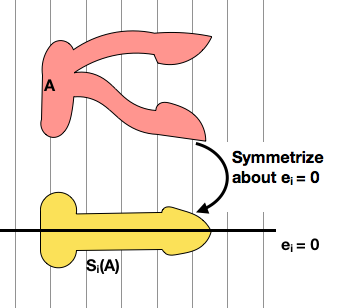
\includegraphics[width=0.5\textwidth]{images/steiner.png}
    \caption{A visualisation of Steiner symmetrization}
    \label{fig: steiner}
\end{figure}

We are now ready to prove the following.
\begin{theorem}
For all $A \subseteq \R^m$ and $\delta > 0$ we have
\[
    \Haus_{\delta}^m=\Haus^m(A)=\lambda_m(A).
\]
\end{theorem}
\begin{proof}
First, we want to prove that
\[
    \lambda_m(A) \le \Haus_{\delta}^m(A)
\]
for all $\delta > 0$ and $A \subseteq \R^m$.

So let $\delta > 0$ and $A \subseteq \R^m$ be given, and let $\{C_i\}_{i \in \N}$ be a $\delta$-covering of $A$. Then
\begin{align*}
    \lambda_m(A) &\le \lambda_m\paren{\bigcup_{i \in \N} C_i} \\
    &\le \sum_{i \in \N} \lambda_m(C_i) \\
    &\le \sum_{i \in \N} \omega_m\paren{\frac{\Diam C_i}{2}}^m
\end{align*}
where the last inequality is due to \cref{thm: isodiametric inequality}. Taking the infimum over all such collections $\{C_i\}_{i \in \N}$ shows the wanted inequality.

Secondly, we show that
\[
    \Haus_{\delta}^m(A) \le \lambda_m(A)
\]
for all $\delta > 0$. Let $\K$ denote the collection of all $m$-dimensional open intervals $I$ of the form $I=(a_1,b_1) \times \dots \times (a_m,b_m)$ for $a_i,b_i \in \R$ with $a_i < b_i$. Then we note that
\[
    \lambda_m(A)=\inf\left\{\sum_{j=1}^{\infty} |I_j| \middle| I_1, I_2, \dots \in \K, A \subseteq \bigcup_{j=1}^{\infty} I_j \right\}
\]
where $|I|=(b_1-a_1)\dots(b_m-a_m)$ denotes the volume of $I$.

Now let $I_1, I_2, \dots \in \K$ be any sequence of $m$-dimensional open intervals such that $A \subseteq \bigcup_{j} I_j$. Now for every bounded open set $U \subseteq \R^m$ and each $\delta > 0$ there exists a pairwise disjoint family of closed balls $B_1, B_2, \dots$ such that $\bigcup_i B_i \subseteq U$, $\Diam B_i < \delta$ for all $i \in \N$ and $\lambda_m(U \setminus \bigcup_i B_i) = 0$. Indeed, there exists a collection $C_1,C_2, \dots $ of closed cubes with pairwise disjoint interiors such that $\Diam C_i < \delta$ for all $i \in \N$ and $U=\bigcup_i C_i$. We write $C_i=(c_i,d_i)^m$ for $c_i,d_i \in \R$ with $c_i<d_i$. Now for each $i \in \N$ there is a ball $B_i \subseteq \mathring{C_i}$ with $\Diam B_i > \frac{d_i-c_i}{2}$ (i.e. half the edge length of $C_i$), for which
\[
    \lambda_m(C_i \setminus B_i) < \paren{1-\frac{\omega_m}{4^m}}\lambda_m(C_i)
\]
and hence
\[
    \lambda_m\paren{U \setminus \bigcup_{i \in \N} B_i} = \lambda_m\paren{\bigcup_{i \in \N} (C_i \setminus B_i) } < \paren{1-\frac{\omega_m}{4^m}}\lambda_m(U).
\]
This implies that for some large enough $N$ we have
\[
    \lambda_m\paren{U \setminus \bigcup_{i = 1}^N B_i} \le \paren{1-\frac{\omega_m}{4^m}}\lambda_m(U).
\]
Since $U \setminus \bigcup_{i = 1}^N B_i$ is open and $\omega_m/4^m\in (0, 1]$ for all $m \ge 0$, we can repeat this argument inductively to obtain the required open balls.

So with $U = I_j$ we take such a collection of open balls $\{B_i\}_{i \in \N}$. Since $\Haus_{\delta}^m$ is absolutely continuous with respect to $\lambda_m$, (i.e. for every $A \subseteq X$ we have $\lambda_m(A) =0 \Rightarrow \Haus_{\delta}^m(A)=0$) we have that
\begin{align*}
    \Haus_{\delta}^m(I_j) &= \Haus_{\delta}^m\paren{\bigcup_{i\in \N} B_i} \\
    &\le \sum_{i=1}^{\infty} \omega_m(\Diam B_i)^m \\
    &= \sum_{i=1}^{\infty} \lambda_m(B_i) \\
    &= \lambda_m\paren{\bigcup_{i\in \N} B_i} \\
    &= \lambda_m(I_j)=|I_j|
\end{align*}
and therefore
\[
    \Haus_{\delta}^m(A) \le \Haus_{\delta}^m\paren{\bigcup_{j \in \N}I_j} \le \sum_{j \in \N} \Haus_{\delta}^m(I_j) \le \sum_{j \in \N}|I_j|.
\]
The second part of this proof thus follows by taking the infimum over all such collections $\{I_j\}_{j \in \N}$.
\end{proof}

\section{Densities}

\begin{definition}
Let $(X,d)$ be any metric space. Then for all outer measures $\mu$ on $X$, $m \in [0, \infty)$, $A \subseteq X$ and $x \in X$ the upper and lower $m$-densities of $A$ at the point $x$ are given by
\begin{align*}
	\Theta^{*m}(\mu,A,x) &= \limsup_{r \to 0^{+}} \frac{\mu (A \cap B_r(a)) }{\omega_{m}r^{m}} \\
	\Theta_{*}^{m}(\mu,A,x) &= \liminf_{r \to 0^{+}} \frac{\mu (A \cap B_r(a)) }{\omega_{m}r^{m}}
\end{align*}
If $\Theta^{*m}(\mu,A,x)=\Theta_{*}^{m}(\mu,A,x)$ then their shared value is called the ($m$-dimensional) density of $A$ at $x$ and denoted by $\Theta^{m}(\mu,A,x)$.
\end{definition}

For the following lemma, we will adopt the notation that if $B=B_r(x) \subseteq X$ is a ball, then $\widehat B=B_{5r}(x)$.
\begin{lemma}[5-times covering lemma]\label{lem: 5-times covering}
If $\m{B}$ is a collection of closed balls in $X$ with $R=\sup\{\Diam B \mid B \in \m B\} < \infty$, then there is a pairwise disjoint subcollection $\m B' \subseteq \m B$ such that
\[
    \bigcup_{B \in \m B} B \subseteq \bigcup_{B \in \m B'} \widehat B.
\]
In fact, an even stronger statement holds, namely, for all $B \in \m B$ there exists a $B' \in \m B'$ such that $B \cap B' \neq \emptyset$ and $\Diam B' \ge \frac{1}{2}\Diam B$ and hence $\widehat B' \supseteq B$.
\end{lemma}
\begin{proof}
For all $i \in \N$ define
\[
    \m B_i := \left\{ B \in \m B \middle| \frac{R}{2^i} < \Diam B \le \frac{R}{2^{i-1}} \right\}
\]
Then clearly $B_i \cap B_j = \emptyset$ for all $i \neq j$, and $\m B = \bigcup_i \m B_i$. We now define another collection $\m B'_i \subseteq \m B_i$ inductively as follows.

For $i=1$, we let $\m B'_i$ be any maximal pairwise disjoint subcollection of $\m B_1$. Such a collection exists by Zorn's lemma applied to $\m C = \{ \m A \mid \m A \text{ is a pairwise disjoint subcollection of } \m B_1\}$, which is partially ordered by inclusion. Furthermore, we see that for any totally ordered subcollection $\m T \subseteq \m C$ we clearly have $\bigcup_{\m A \in \m T} \m A \in \m C$ so Zorn's lemma does indeed apply. Moreover, in a general metric space, the collection $\m B'_1$ could be uncountable. But in a separable metric space all pairwise disjoint collections of balls must be countable.

Next, for every $i \ge 2$ assume that $\m B'_1 \subseteq \m B_1, \dots, \m B'_{i-1} \subseteq \m B_{i-1}$ have been defined. Then we let $\m B'_i$ be a maximal pairwise disjoint subcollection of 
\[
    \left\{B \in \m B_i \middle| B \cap B' = \emptyset, \text{ when } B' \in \bigcup_{j=1}^{i-1} \m B'_j\right\}.
\]
Another Zorn's lemma argument guarantees such a maximal collection exists. Now if $i \ge 1$ and $B \in \m B_i$ we have $B \cap B' \neq \emptyset$ for some $B' \in \bigcup_{j=1}^i \m B'_j$, otherwise this would contradict maximality of $\m B'_i$. For such a pair $B$ and $B'$ we have
\[
    \Diam B \le R/2^{i-1}=2R/2^i \le 2 \Diam B'
\]
so that \cref{lem: 5-times covering} holds, and in particular $B \subseteq \widehat B'$.
\end{proof}

In the following corollary we say that $A \subseteq X$ is \emph{covered finely} by a collection $\m B$ of balls, if for all $x \in A$ and all $\varepsilon > 0$ there is a ball $B \in \m B$ with $x \in B$ and $\Diam B < \varepsilon$.
\begin{corollary}\label{cor: fine cover}
Let $\m B$ be as in \cref{lem: 5-times covering}. Then if $A \subseteq X$ is covered finely by $\m B$ and $\m B' \subseteq \m B$ is any pairwise disjoint subcollection of $\m B$ satisfying \cref{lem: 5-times covering}, then for each finite subcollection $\{B_1, \dots, B_N\} \subseteq \m B'$ we have
\[
    A \setminus \bigcup_{i=1}^N B_i \subseteq \bigcup_{B \in \m B' \setminus \{B_1, \dots, B_N\}} \widehat B.
\]
\end{corollary}
\begin{proof}
Let $x \in A \setminus \bigcup_{i=1}^N B_i$. Then since $A$ is covered finely by $\m B$ and $X \setminus \bigcup_{i=1}^N B_i$ is open, there is a $B \in \m B$ with $B \cap \paren{\bigcup_{i=1}^N B_i} = \emptyset$ and $x \in B$, and by \cref{lem: 5-times covering} there is a $B' \in \m B'$ with $B' \cap B \neq \emptyset$ such that $B \subseteq \widehat{B'}$. This implies that $B' \cap B_i \neq \emptyset$ for all $i =1, \dots, N$ so $x \in \bigcup_{B' \in \m B' \setminus \{B_1, \dots, B_N \}} \widehat{B'}$.
\end{proof}

\begin{theorem}\label{thm: upper density connection}
Let $\mu$ be a Borel regular measure on $X$, $t \ge 0$ and $A_1 \subseteq A_2 \subseteq X$. Then if
\[
    \Theta^{*n}(\mu,A_2,x) \ge t,
\]
for all $x \in A_1$, then
\[
    t\Haus^m(A_1) \le \mu(A_2)
\]
\end{theorem}
\begin{proof}
If $\mu(A_2)=\infty$ or $t=0$, the result is trivial, so assume that $\mu(A_2)<\infty$ and $t>0$.

Let $\tau \in (0,t)$ be given, and assume that $\Theta^{*m}(\mu,A_2,x) > \tau$ for all $x \in A_1$. For any $\delta > 0$, define $\m B_{\delta}$ by
\[
    \m B_{\delta} = \left\{ B_r(x) \middle| x \in A_1, r \in (0,\delta/2), \frac{\mu(A_2 \cap B_r(x))}{\omega_mr^m} \ge \tau \right\}
\]
This collection $\m B_{\delta}$ covers $A_1$ finely, so there is a subcollection $\m B' \subseteq \m B_{\delta}$ such that \cref{lem: 5-times covering} holds. Then since $\mu(A_2\cap B) > 0$ for each $B \in \m B_{\delta}$ and since 
\[
    \sum_{i=1}^{N} \mu(A_2 \cap B_i) = \mu\paren{A_2 \cap \paren{\bigcup_{i=1}^N B_i } } \le \mu(A_2) < \infty
\]
for all balls $B_1, \dots, B_N \in \m B'$, it follows that $\m B'$ is a countable collection $\{B_{r_1}(x_1), B_{r_2}(x_2), \dots\}$ and hence \cref{cor: fine cover} implies that
\[
    A_1 \setminus \bigcup_{i=1}^N B_{r_i}(x_i) \subseteq \bigcup_{i=N+1}^{\infty} B_{5r_i}(x_i)
\]
for all $N \ge 1$.

Furthermore, by the construction of $\m B_{\delta}$, we have that
\[
    \tau \sum_{i=1}^{\infty} \omega_m r_i^m \le \sum_{i=1}^{\infty} \mu(A_2 \cap B_{r_i}(x_i)) = \mu\paren{A_2 \cap \paren{\bigcup_{i=1}^{\infty} B_{r_i}(x_i) }} \le \mu(A_2) < \infty.
\]
Therefore
\[
    A_2 \subseteq \paren{\bigcup_{i=1}^N B_{r_i}(x_i) } \cup \paren{\bigcup_{i=N+1}^{\infty} B_{5r_i}(x_i)}
\]
and hence by the definition of $\Haus^m_{\delta}$, we have
\[
    \Haus^m_{5\delta}(A_1) \le \sum_{i=1}^N \omega_m r_i^m + 5^m \sum_{i=N+1}^{\infty} \omega_m r_i^m.
\]
So by letting $N \to \infty$ we get that
\[
    \tau \Haus^m_{5\delta}(A_1) \le \mu(A_2)
\]
And then letting $\delta \to 0$, and then $\tau \to t$ the result follows.
\end{proof}

\begin{theorem}[Upper density theorem]\label{thm: upper density theorem}
If $\mu$ is a Borel regular measure on $X$ and if $A \subseteq X$ is $\mu$-measurable with $\mu(A)<\infty$, then
\[
    \Theta^{*m}(\mu,A,x)=0
\]
for $\Haus^m$-a.e. $x \in X \setminus A$.
\end{theorem}
\begin{proof}
For a given $t > 0$, define
\[
    S_t:=\{x \in X \setminus A \mid \Theta^{*m}(\mu,A,x) \ge t \}
\]
and let $C$ be any closed subset of $A$. Then, since $X \setminus C$ is open, and $S_t \subseteq X \setminus A \subseteq X \setminus C$ we have
\[
    \Theta^{*m}(\mu,A\cap(X \setminus C),x) = \Theta^{*m}(\mu,A,x) \ge t
\]
for all $x \in S_t$. Thus we can apply \cref{thm: upper density connection} with $\mu \llcorner A, S_t$ and $X \setminus C$ in place of $\mu,A_1$ and $A_2$ to obtain that $t\Haus^m(S_t) \le \mu(A\setminus C)$ for each closed set $C \subseteq A$.

Now since $\mu$ is an outer measure on a metric space $X$, it has the Radon measure property that $\mu(A) = \sup_C\{\mu(C)\}$ where the supremum is taken over all closed subsets, $C$, of $A$. Therefore we can find a sequence $\{C_i\}_{i \in \N}$ such that $C_i \subseteq A$ are closed for all $i$, and such that $\mu(A \setminus C_i) \to 0$ as $i \to \infty$, which implies that $\Haus^m(S_t)=0$. Finally letting $t \to \infty$ we conclude that
\[
    \Haus^m(\{x \in X \setminus A \mid \Theta^{*m}(\mu,A,x)>0 \} ) = 0,
\]
which finishes the proof.
\end{proof}


\section{The Area and Co-Area Formulae}
Next we want to develop a generalized area formula similar to the one in the introduction. We shall need the following theorem, which we will not prove.
\begin{theorem}[Rademacher's Theorem]
If $f$ is Lipschitz on $\R^n$, then $f$ is differentiable $\Haus^n$-a.e. i.e. the gradient $\nabla f(x) = (D_1f(x), \dots, D_nf(x))$ exists and
\begin{align*}
    \lim_{y \to x} \frac{f(y) - f(x) - \nabla f(x)(y-x)}{|y-x|} = 0
\end{align*}
for $\Haus^n$-a.e. $x \in \R^n$.
\end{theorem}

It is well known that for a linear map $L: \R^m \to \R^m$, and $A \subseteq \R^n$ we have that $\lambda_m(L(A)) = |\det L| \lambda_m(A)$. We want to develop a counterpart to this.


If $L: \R^n \to \R^m$ is a linear mapping, we define the Jacobian determinant, $J_L$ of $L$ as
\begin{align*}
    J_L=\sqrt{\det(L^* \circ L)}
\end{align*}

Now let $f=(f_1, \dots, f_m):\R^n \to \R^m$, for $n \le m$ be a Lipschitz mapping. By Rademacher's theorem, $f$ is differentiable at $\lambda_n$-a.e. $x \in \R^n$. Hence the Jacobian matrix $Df(x)$ exists and can be expressed as a matrix
\begin{align*}
    Df(x) = \begin{pmatrix}
        \frac{\partial f_1}{\partial x_1} & \dots & \frac{\partial f_1}{\partial x_n} \\
        \vdots & \ddots & \vdots \\
        \frac{\partial f_m}{\partial x_1} & \dots & \frac{\partial f_m}{\partial x_n} \\
    \end{pmatrix}
\end{align*}
at $\lambda_n$-a.e. $x \in \R^n$.

Now $Df(x)$ is a linear mapping whenever it exists, so we can similarly define the Jacobian determinant, $J_f$ of $f$ at a point $x$ where $f$ is differentiable as
\begin{align*}
    J_f:=J_{Df}
\end{align*}

\begin{lemma}
Let $L:\R^n \to \R^m$, $n \le m$ be a linear map. Then
\begin{align*}
    \Haus^n(LA)=J_L\Haus^n(A)
\end{align*}
for all $A \subseteq \R^n$.
\end{lemma}
\begin{proof}
Since $L$ is linear, $L(\R^n) \subseteq F$ for some $n$-dimensional subspace, $F \subseteq \R^m$. Therefore we can choose an orthogonal transformation $q:\R^m \to \R^m$ such that $q(F)=\R^n \times \{0\}$. We can further define a projection $p:\R^n\times \R^k =\R^m \to \R^n$ such that $p(x,y)=x$ for $(x,y) \in \R^n \times \R^k$. We then see that $p \circ q \circ L:\R^n \to \R^n$ and thus by the discussion at the beginning of the section, $\Haus^n((p\circ q \circ L)(A))=|\det(p \circ q \circ L)|\Haus^n(A)$ for all $A \subseteq \R^n$. Using the adjoint, we get that $(p\circ q \circ L)^*(p\circ q \circ L)=L^*\circ q^* \circ (p^* \circ p) \circ q \circ L$. But $p^* \circ p$ is the identity on $\R^n \times \{0\}$, and $q$ is orthogonal so $q^* \circ q$ is the identity on $\R^m$, hence $L^*\circ q^* \circ (p^* \circ p) \circ q \circ L=L^* \circ L$. Therefore $|\det(p \circ q \circ L)|=\sqrt{\det (L^* \circ L)}=J_L$. This finishes the proof.
\end{proof}

Now, we can generalize this to Lipschitz functions, to get the following theorem, which can be proved by an approximation argument based on the linear case
\begin{theorem}[Area formula]\label{thm: area formula}
If $f:\R^n \to \R^m$ is Lipschitz and injective, then
\begin{align*}
    \Haus^n(f(A)) = \int_A J_f \, d\Haus^n.
\end{align*}
for all $\Haus^n$-measurable $A \subseteq \R^n$.
\end{theorem}

\begin{example}
Let $g: \R^m \to \R$ be Lipschitz, and define $f:\R^m \to \R^{m+1}$ by $f(x)=(x,g(x))$. Then
\begin{align*}
    Df=\begin{pmatrix} I \\ \nabla g \end{pmatrix}
\end{align*}
and hence $J^2_f=1+|\nabla g|^2$. Given an open set $U \subseteq \R^m$, the graph, $\Gamma$, of $g$ over $U$ is given by
\begin{align*}
    \Gamma = \{ (x,g(x)) \mid x \in U \}
\end{align*}
and therefore
\begin{align*}
    \Haus^m(\Gamma) = \int_U \sqrt{1 + |\nabla g|^2} d\Haus^m(x).
\end{align*}
This looks strikingly similar to \eqref{eq: 3 area formula}, so we are going in the right direction.
\end{example}

We state without proof the following generalisations of the area formula.

\begin{theorem}[Area formula]
Suppose $f: \R^n \to \R^m$ is Lipschitz and $n \le m$. If $A \subseteq \R^n$ is $\lambda_n$-measurable then
\begin{align*}
    \int_A J_f(x)\, d\lambda_n(x) = \int_{\R^m} \Haus^0(f^{-1}(\{y\} \cap A) \, d\Haus^n(y).
\end{align*}
Note that $\Haus^0$ is the counting measure.
\end{theorem}

\begin{theorem}
Suppose $f: \R^n \to \R^m$ is Lipschitz and $n \le m$.
If $g$ is an $\lambda_n$-integrable function, then
\begin{align*}
    \int_{\R^n} g(x)J_f(x) \, d\lambda_n = \int_{\R^m} \sum_{x \in f^{-1}(y)} g(x) \, d\Haus^n(y).
\end{align*}
\end{theorem}

Next we briefly discuss the co-area formula, which is generalization of Fubini's theorem.

\begin{theorem}[The co-area formula]
Let $n \ge m$ and $f:\R^n \to \R^m$ be Lipschitz. Then for every $\lambda_m$-measurable set $A \subseteq \R^n$ we have
\begin{align*}
    \int_A J_f(x) \, d\lambda_n(x) = \int_{\R^m} \Haus^{n-m}(A \cap f^{-1}(y)) \, d\lambda_m(y)
\end{align*}
\end{theorem}

\begin{theorem}[Change of variables]
Let $f: \R^n \to \R^m$, for $n \ge m$ be Lipschitz. Then for every $\lambda_n$ integrable function $g:\R^n \to \R$, $g|_{f^{-1}(y)}$ is $\Haus^{n-m}$ integrable for $\lambda_m$-a.e. $y \in \R^m$ and
\begin{align*}
    \int_{\R^n} g(x)J_f(x)\, d\lambda_n(x) = \int_{\R^m} \paren{ \int_{ f^{-1}(y) } g\, d\Haus^{n-m} } \, d\lambda_m(y)
\end{align*}
\end{theorem}

\section{Sobolev Spaces}
We shall briefly discuss the theory of Sobolev spaces, which we will used to prove the Allard Regularity \cref{thm: allard}. See \cite{kinnunen20} for reference.

\begin{definition}
Let $u \in L_{loc}^1(\Omega)$ for some open set $\Omega \subseteq \R^n$, and let $\alpha \in \N^n$ be a multi-index. Then $v \in L_{loc}^1(\Omega)$ is the weak partial derivative of order $\alpha$ of $u$, written $D^{\alpha}u=v$ if
\[
    \int_{\Omega} u D^{\alpha}\varphi\, dx = (-1)^{|\alpha|} \int_{\Omega} v\varphi\, dx
\]
for all $\varphi \in C_c^{\infty}(\Omega)$
\end{definition}

Then we can define the Sobolev spaces as
\begin{definition}
For all open sets $\Omega \subseteq \R^n$, define the Sobolev space by
\[
    W^{k,p}(\Omega) = \{ u \in L^p(\Omega) \mid D^{\alpha} u \in L^p(\Omega), |\alpha| \le k \}.
\]
\end{definition}

For every $u \in W^{k,p}(\Omega)$ we define the Sobolev norm by
\[
    \Vert u \Vert_{W^{k,p}(\Omega)} := \paren{ \sum_{|\alpha| \le k} \int_{\Omega} \left| D^{\alpha}u \right|^p\, dx }^{\frac{1}{p}}
\]
for $1\le p < \infty$, and otherwise
\[
    \Vert u \Vert_{W^{k,\infty}(\Omega)} := \sum_{|\alpha| \le k} \esssup_{\Omega} \left| D^{\alpha}u \right|,
\]
where $\esssup$ denotes the essential supremum, that is, for every measurable function $f:(X,\mu) \to \R$ where $\mu$ is some measure, the essential supremum of $f$ is defined as the smallest number $\kappa$ for which
\[
    \mu(f^{-1}(\kappa, \infty)) = \mu(\{x \in X \mid f(x) > \kappa\}) = 0.
\]
If no such $\kappa$ exists, we define the essential supremum to be $\infty$.

\begin{theorem}[Poincaré inequality]\label{thm: poincare inequality}
Let $1 \le p < \infty$ be given, and $\Omega \subseteq \R^n$ be open and bounded. Then there is some constant $C=C(p)$ for which
\[
    \int_{\Omega} |u|^p \, dx \le C \Diam(\Omega)^p \int_{\Omega} |Du|^p\, dx
\]
for every $u \in W_0^{1,p}(\Omega)$ ($=$ the completion of $C_c^{\infty}(\Omega)$ with respect to the Sobolev norm).
\end{theorem}
\begin{proof}
We prove the theorem for $u \in C_c^{\infty}(\Omega)$, and then since $W_0^{1,p}(\Omega)$ can be approximated by functions in $C_c^{\infty}(\Omega)$ (see \cite{kinnunen20} theorem 1.18), the theorem follows by an approximation argument.

So let $u \in C_c^{\infty}(\Omega)$, and $y \in \Omega$. Then letting $a_i := y_i - \Diam(\Omega)$ and $b_i = y_i + \Diam(\Omega)$ for all $i=1, \dots, n$, we have
\[
    \Omega \subseteq \prod_{i=1}^n [a_i, b_i].
\]
Then as in the proof of \cite{kinnunen20} theorem 2.2, we get
\begin{align*}
    |u(x)| &\le \int_{a_i}^{b_i} |Du(x_1, \dots, t_i, \dots, x_n)| \, dt_i \\
    &\le (2 \Diam(\Omega))^{1-\frac{1}{p}} \paren{ \int_{a_i}^{b_i} |Du(x_1, \dots, t_i, \dots, x_n)|^p \, dt_i }^{\frac{1}{p}}
\end{align*}
for all $i = 1, \dots, n$. This allows us to use the Hölder inequality, and write
\begin{align*}
    \int_{\Omega} |u(x)|^p \, dx &= \int_{a_1}^{b_1} \dots \int_{a_n}^{b_n} |u(x)|^p \, dx_1\dots dx_n \\
    &\le (2\Diam(\Omega))^{p-1} \int_{a_1}^{b_1} \dots \int_{a_n}^{b_n} \int_{a_1}^{b_1} |Du(t_1, x_2, \dots, x_n)|^p \, dt_1 dx_2\dots dx_n \\
    &\le (2\Diam(\Omega))^{p} \int_{a_1}^{b_1} \dots \int_{a_n}^{b_n} |Du(t_1, x_2, \dots, x_n)|^p \, dt_1\dots dx_n \\
    &= (2\Diam(\Omega))^{p} \int_{\Omega} |Du(x)|^p \, dx
\end{align*}
which finishes the proof.
\end{proof}

A fact that we shall use later in the Allard regularity theorem is the following Rellich-Kondrachov Compactness theorem, which we state without a proof. See \cite{gt01} pp 167--168.
\begin{theorem}[Rellich-Kondrachov compactness theorem]\label{thm: Rellich-Kondrachov}
Let $\Omega\subseteq \R^n$ be open. Then the Sobolov space $W^{1,p}(\Omega)$ is compactly embedded in $L^q(\Omega)$ for all $q < \frac{np}{n-p}$ if $1\le p < n$.
\end{theorem}

Notice that an embedding is compact if and only if the identity operator is a compact operator. Thus the Rellich-Kondrachov compactness theorem implies that any uniformly bounded sequence in $W^{1,p}(\Omega)$ has a subsequence that converges in $L^p(\Omega)$.